%
%>>>>>>>>>>>>>>>>>>>>>>>>>>>>>>>>>>>>>>>>>>>>>>>>>>>>>>>>>> The O2/FLP subsystem 
%

The major upgrade of the ALICE experimental apparatus, the resulting dramatic increase of the performance requirements, and the advancement of computing technology have been the major reasons for the design and the implementation of a new computing system called $O^2$ divided in three parts: FLP, EPN and PDP. 

The $O^2$/FLP subsystem includes the First-Level Processors (FLPs) detector read-out farm, the data quality control system and the services for control, configuration, monitoring, logging, and bookkeeping. 
%
%>>>>>>>>>>>>>>>>>>>>>>>>>>>>>>>>>>>>>>>>>>>>>>>>>>>>>>>>>> The FLP farm 
%
\subsubsection{The FLP detector read-out farm}
The read-out farm includes 198 nodes and 490 readout cards (distributed as shown in Table~\ref{tab:flp_farm_links}) for transferring the data from all detectors to the $O^2$ system.

\begin{table}[h!]
\centering
\caption{FLP read-out farm used to transfer the data from the detectors to the $O^2$ system.}
\label{tab:flp_farm_links}
\begin{tabular} { l l r r l r r r}
\hline
Detector &  Link 	&  \multicolumn{2}{c}{Read-out links}  &  \multicolumn{2}{c}{Read-out boards} & Read-out \tabularnewline
         &  type 	& DDL   	& GBT       & C-RORC& CRU	& nodes FLPs \tabularnewline
\hline
CPV     & DDL           &               & ?         &       & 1         &   1 \tabularnewline
CTP     & GBT           &               & 14        &       & 1         &   1 \tabularnewline
DCS     &               &               &           &       &           &   1 \tabularnewline
EMC     & DDL           & 40            &           & 8     &           &   2 \tabularnewline
FIT     & GBT           &               & 34        &       & 3         &   1 \tabularnewline
HMP     & DDL           & 14            &           & 4     &           &   2 \tabularnewline
ITS     & GBT           &               & 495       &       & 24        &  12 \tabularnewline
MCH     & GBT           &               & 550       &       & 30        &  11 \tabularnewline
MFT     & GBT           &               & 304       &       & 11        &   5 \tabularnewline
MID     & GBT           &               & 32        &       & 2         &   1 \tabularnewline
PHS     & DDL           & 16            &           & 4     &           &   2 \tabularnewline
TOF     & GBT           &               & 72        &       & 4         &   2 \tabularnewline
TPC     & GBT           &               & 5832      &       & 361       & 145 \tabularnewline
TRD     & Custom        &               & 1044      &       & 36        &  12 \tabularnewline
ZDC     & GBT           &               & 1         &       & 1         &   1 \tabularnewline
Total   &               & 76            & 8928      & 16    & 474       & 198 \tabularnewline
\end{tabular}
\end{table}
The total nominal read-out performance amounts to 3.4~TB/s from the detector electronics to the read-out boards and the FLP servers. Most of the detectors use the new GBT~\cite{ref_GBT} link and the Common Read-out Unit (CRU)~\cite{ref_CRU_HW, ref_CRU_FW} adopted for this upgrade. The system is also backward compatible with the Detector Data Link (DDL)~\cite{ref_DDL} and the Common Read-Out Receiver Card (C-RORC)~\cite{ref_RORC} used during the LHC Run 1 and 2. 

The server selected for the FLPs is the Dell Poweredge R740. The selection has been done after numerous hardware and software tests~\cite{ref_FLP} and a competitive tender. Each FLP is equipped with 96~GB of DDR memory and 2~CPUs. The CPUs are of two different flavours of the Intel Cascade Lake generation (the Silver 4210 or the Gold 6230 with 10 or 20 hardware cores respectively) depending on the processing needs of the detector. Each FLP hosts up to three CRUs, up to four CRORCs and one Infiniband network interface, each using one PCIe Gen3 x16 slot. The readout software performance allows data to be transferred from 3~CRUs simultaneously at the maximum PCIe Gen3 performance for a total of 330~Gb/s.

The first layer over the PCIe interface to the cards is the PDA (Portable Driver Architecture) UIO (Userspace IO) kernel module~\cite{ref_PDA}. PDA also provides a userspace library in C~\cite{ref_PDA_lib} which supports PCIe device enumeration and provides a handle to PCI devices.
The read-out software includes the readout program and the readoutCard library~\cite{ref_readout} which orchestrate the simultaneous data transfers from the GBT links to the FLP memory and from the memory to the network interface as shown in Fig.\ref{fig_RO}. 
%
\begin{figure}[!h]
\centering
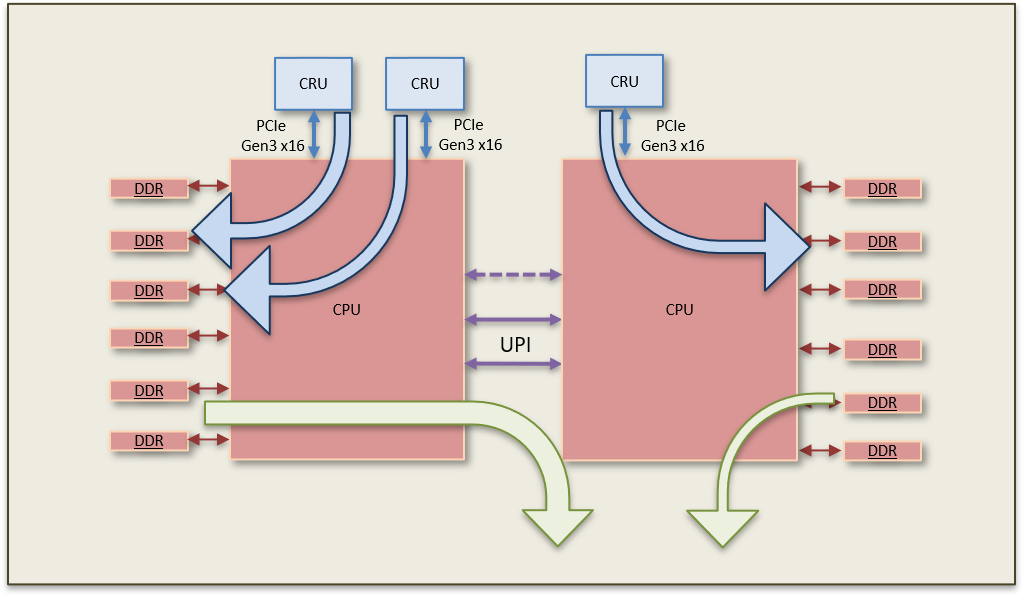
\includegraphics [width=100mm] {o2_flp/Readout_dataflows.png}
\caption{Simultaneous dataflows inside the FLP from the CRUs to the DDR memories and from the memory to the Infiniband network to the EPN farm.}
\label{fig_RO}
\end{figure}
%
 
%
%>>>>>>>>>>>>>>>>>>>>>>>>>>>>>>>>>>>>>>>>>>>>>>>>>>>>>>>>>> The data quality control 
%
\subsubsection{The data quality control}
The online execution of the calibration and the reconstruction and the replacement of the raw input data by reconstructed data, make the need for a reliable data Quality Control (QC) even more essential than usual. Its main motivations are to identify and help overcome problems during data taking and check that the data processing behaves as expected, thus ensuring good quality data for physics analyses.

The $O^2$  QC system \cite{ref_QC} is a distributed software as shown in Fig.\ref{fig_QC}.
    Data samples are selected following a pseudo-random sampling and configurable policies at key points in the data-flow and are dispatched to local (on the FLPs and the EPNs) or remote (on QC servers) QC tasks executing detector-specific algorithms. Their results are published as QC Objects, typically ROOT~\cite{ref_ROOT} histograms. The results of the QC tasks running in parallel on many nodes are assembled by the mergers.  
    Traditional or machine-learning-based checkers evaluate the quality of the objects and produce QC qualities. Finally the QC Objects and the Qualities are stored in the QC repository. This database uses the same technology as the Calibration and Condition DataBase of ALICE $O^2$. The Post-processing component encompasses asynchronous tasks such as correlation and trending of data derived from QC Objects and Qualities and triggered periodically, manually or on certain events (e.g. start of run or end of fill).
    QC and Quality Objects are accessible to shifters and experts through a web-based QC GUI.
%\end{itemize}
%
\begin{figure}[!h]
\centering
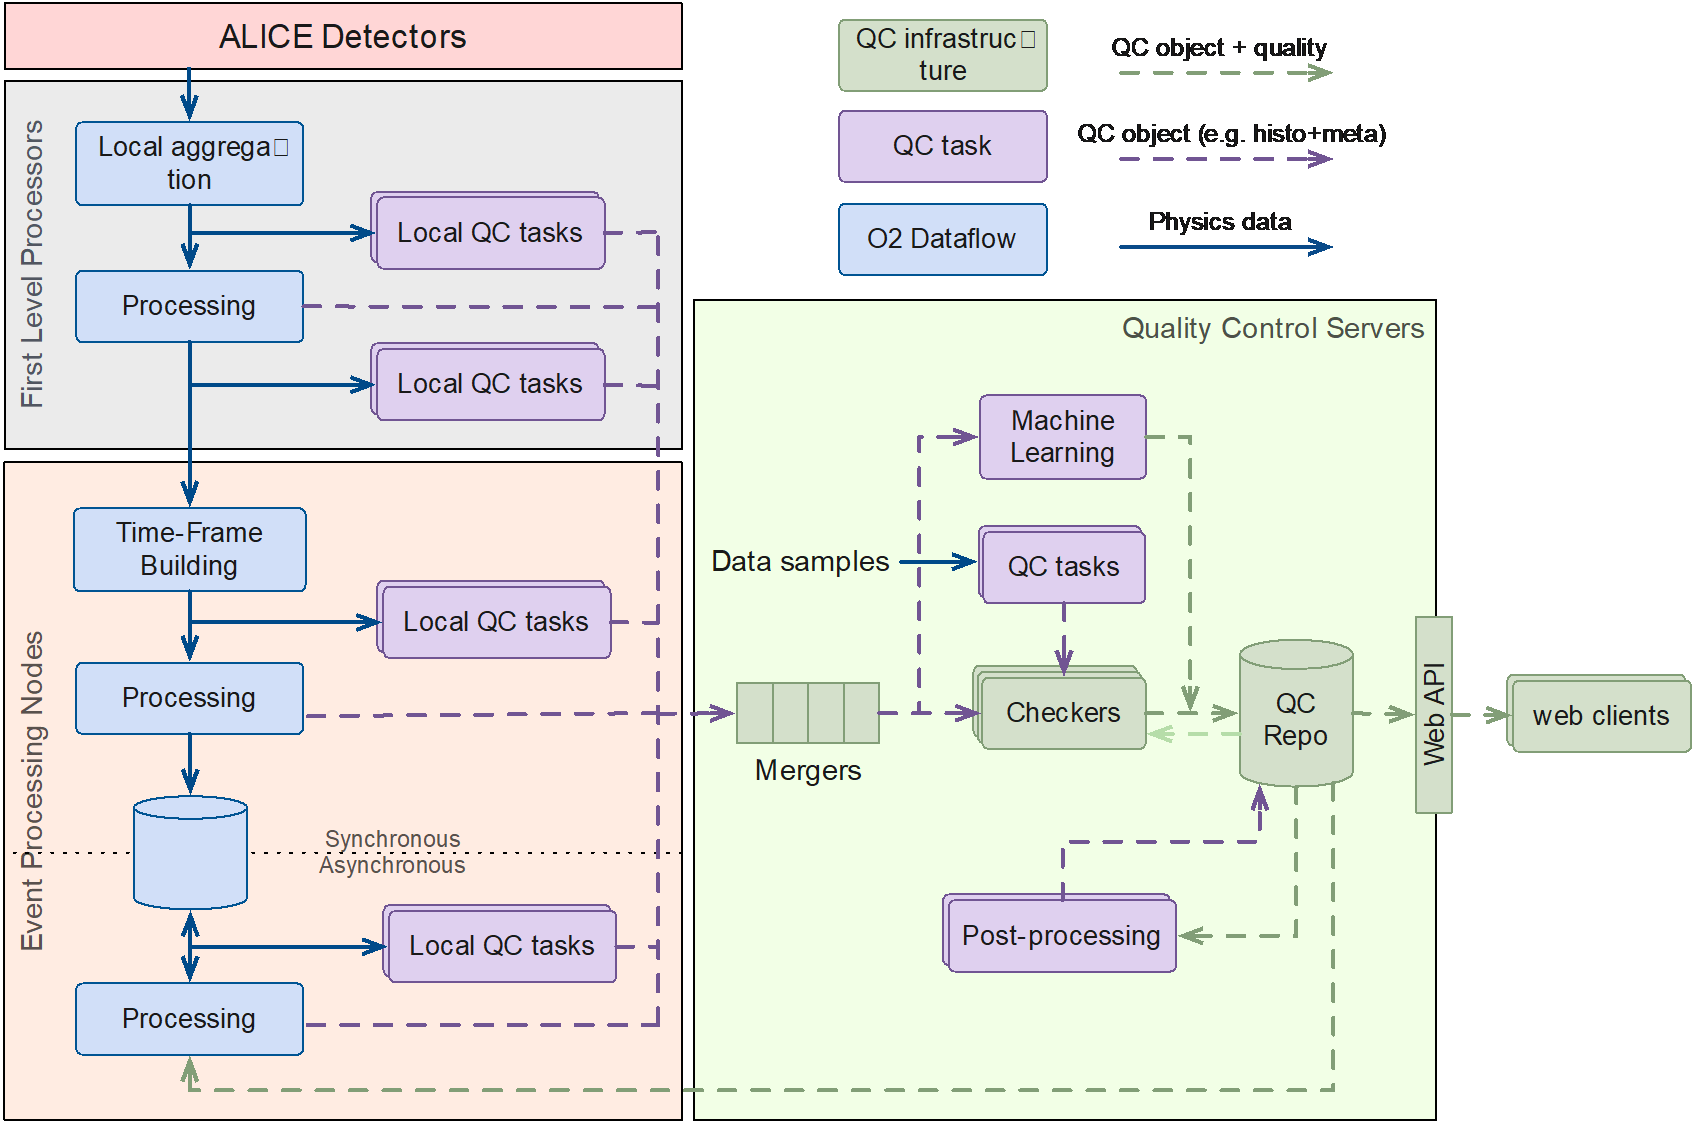
\includegraphics [width=100mm] {o2_flp/QC_Design.png}
\caption{$O^2$ Quality Control design.}
\label{fig_QC}
\end{figure}
%
%>>>>>>>>>>>>>>>>>>>>>>>>>>>>>>>>>>>>>>>>>>>>>>>>>>>>>>>>>> The services 
%
\subsubsection{The services}
%
%>>>>>>>>>>>>>>>>>>>>>>>>>>>>>>>>>>>>>>>>>>>>>>>>>>>>>>>>>> WebUI
\paragraph {Web User Interface framework}
Overview
The Web User Interface (Web UI) framework provides the core functionalities and building blocks to easily create rich web applications.
The server side features REST and WebSocket API, the authentication via CERN single sign-on and the authorisation using CERN e-groups.
The client-side features user interface Cascading Style Sheet building blocks, asynchronous data fetching (Ajax) and bi-directional socket (WebSockets).

%>>>>>>>>>>>>>>>>>>>>>>>>>>>>>>>>>>>>>>>>>>>>>>>>>>>>>>>>>> Control and configuration 
%
\paragraph{Control and configuration}
The ALICE Experiment Control System (AliECS) \cite{ref_aliecs} integrates the experiment control and configuration, the FLP farm control and a high-level control interface to the $O^2$/EPN cluster as shown in Fig~\ref{fig_aliecs}. It implements a distributed state machine to represent the aggregated state of the constituent $O^2$ processes of a data-driven workflow. Furthermore, it allows reconfiguration of running processes and simultaneous operation of multiple worflows, with easy reallocation of resources among workflows. Finally, it reacts promptly to inputs, handling events from the user, the LHC, the trigger system, the DCS, and the cluster itself with a high degree of autonomy. 

AliECS uses FairMQ, part of ALFA \cite{ref_alfa}, which is the common $O^2$ transport layer for physics data.   
Apache Mesos~\cite{ref_mesos} is a cluster resource management system, which facilitates the management of O2/FLP components, resources and tasks inside the O2/FLP facility, 
effectively enabling the developer to program against the datacenter (i.e., the O2/FLP facility at LHC Point 2) as if it was a single pool of resources. 

AliECS interfaces with Consul~\cite{ref_consul}, a key-value store which acts as the system’s configuration repository. The design also includes interfacing with information sources from the LHC, 
the trigger system, and the DCS. Once acquired by the AliECS core, configuration information is processed into an in-memory hierarchical key-value store, and from there it is
fed into a template system in order to generate task deployment and configuration structures.

Most components of AliECS are written in Go~\cite{ref_go}, a statically typed general purpose programming language in the tradition of C, which is particularly suitable for distributed system development because of its advanced synchronization and threading facilities.

\begin{figure}[!h]
\centering
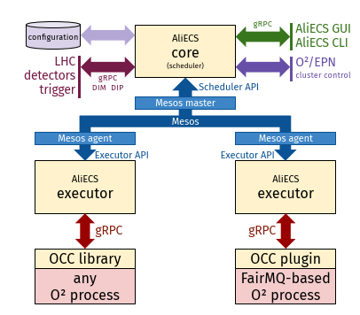
\includegraphics [width=100mm] {o2_flp/AliECS_Design.png}
\caption{AliECS design.}
\label{fig_aliecs}
\end{figure}

%
%>>>>>>>>>>>>>>>>>>>>>>>>>>>>>>>>>>>>>>>>>>>>>>>>>>>>>>>>>> Monitoring 
%
\paragraph{Monitoring}
The monitoring subsystem \cite{ref_monitor1, ref_monitor2} provides a complete overview of the overall system health, detects performance degradation and component failures by collecting, processing, storing and visualising values from hardware and software sensors and probes. As presented in Fig.~\ref{fig_monitoring}, metrics are sent to the system from both Telegraf \cite{ref_telegraf} (for system metrics) and the C++ monitoring library (via Telegraf, for application metrics). These metrics are processed in an Apache Kafka \cite{ref_Kafka} cluster and later written to InfluxDB \cite{ref_influxdb} time-series database for permanent storage.

InfluxDB time-series database supports downsampling which decreases the value resolution over time bringing down the total database size. It is planned to keep high resolution metrics for several days. After that time metrics will be downsampled in order to decrease the number of points and store them until the end of the calendar year. 

The system includes a data visualisation interface based on Grafana \cite{ref_grafana} and channels to email or mattermost for alarms and reporting.
\begin{figure}[!h]
\centering
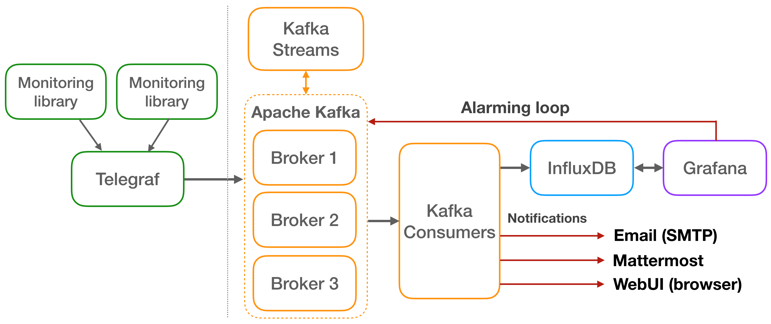
\includegraphics [width=100mm] {o2_flp/Monitoring_Design.png}
\caption{The $O^2$ computing system monitoring design.}
\label{fig_monitoring}
\end{figure}

%
%>>>>>>>>>>>>>>>>>>>>>>>>>>>>>>>>>>>>>>>>>>>>>>>>>>>>>>>>>> Logging 
%
\paragraph{Logging}
The logging system has been adapted from the ALICE Run 2 DAQ software \cite{ref_logging}. A new web-based user interface has been developed in addition to the existing GUIs.
%
%>>>>>>>>>>>>>>>>>>>>>>>>>>>>>>>>>>>>>>>>>>>>>>>>>>>>>>>>>> Bookkeeping 
%
\paragraph{Bookkeeping}
A new bookkeeping system called Jiskefet \cite{ref_bookkeeping} has been developed. It unifies two functionalities: gathering, storing and presenting metadata associated with the operations of the ALICE experiment and tracking the asynchronous processing of the physics data. The front end is based on the WebUI framework like the other applications and is adaptive to various clients such as tablets, mobile devices and other screens. The back end includes an OpenAPI specification based REST API and a relational database.

